\documentclass{beamer}

\usepackage{luatexja}
\usepackage{hyperref}
\hypersetup{unicode}
\usepackage{bm}

\usetheme{Darmstadt}
\usecolortheme{dolphin}
\usefonttheme[onlymath]{serif}

%-----------------------------------------------------------

\AtBeginSection[]{
  \begin{frame}<beamer>
    \tableofcontents[sectionstyle=show/hide,subsectionstyle=hide/show/hide]
    \begin{figure}
      \flushright{
        
\includegraphics[width=3cm]{image/iwbtg.pdf}
      }
    \end{figure}
  \end{frame}
  \addtocounter{framenumber}{-1}
}

%-----------------------------------------------------------

\title{タイトル}
\author{@asi1024}
\institute{Kyoto Univ. Informatics and Mathematical Science 2nd}
\date{\today}

\begin{document}

\frame{\titlepage}
\frame{
  \tableofcontents[sectionstyle=show,subsectionstyle=hide]
}

\section{はじめに}

\subsection{自己紹介}
\frame{
  \frametitle{自己紹介}
  \begin{itemize}
  \item ID: asi1024
  \item Position: 前会計
  \item Twitter: asi1024
  \item KMCでの活動: 競技プログラミングなど\\ \\
  \item ICPCのチームメイトを求めて京都大学にやってきた
  \item ICPCのチームメイトを求めてKMCにやってきた
  \item 本当は大学に入ったら弓道をやるつもりだった
  \end{itemize}
}

\subsection{この講座の目的}
\frame{
  \frametitle{この講座の目的}
  \itemize{
  \item データ構造「ヒープ」について知ってもらう\\ \\
    \itemize{
    \item 半分は実用性
    \item 半分は理論的興味\\
    }
  }
}


\section{グラフとツリー}

\subsection{What's グラフ?}
\frame{
  \frametitle{グラフ}
  \begin{block}{graph}
    \alert{グラフ}は有限集合$V,E$と関数$\Psi$の3つ組で定義され,\\ \\
    無向グラフの場合,
    \[ \Psi: E \rightarrow \{ X \subset V : |X| = 2 \} \]
    有向グラフの場合,
    \[ \Psi: E \rightarrow V \times V\]
     
  \end{block}
}

\frame{
  \begin{exampleblock}{グラフの例}
    左が有向グラフ,右が無向グラフ
    \center{
      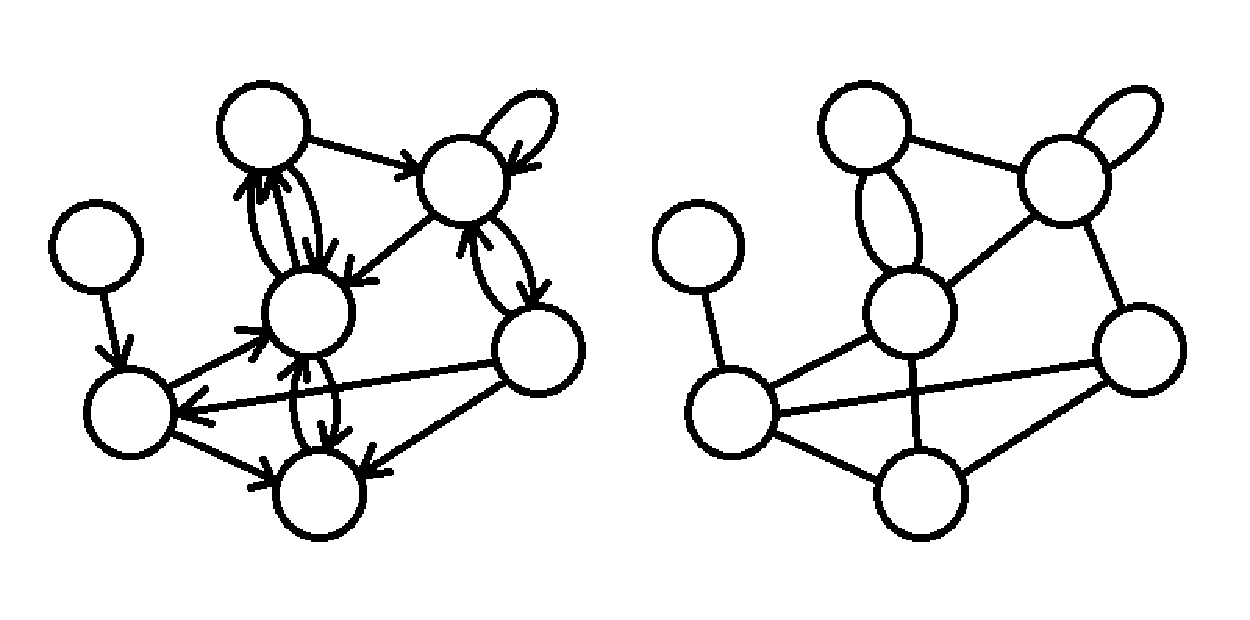
\includegraphics[width=8cm]{image/graph01.pdf}
    }
  \end{exampleblock}
}
    
\subsection{単純グラフ}
\frame{
  \frametitle{単純グラフ}
  \begin{block}{simple graph}
    自己ループと多重辺を持たないグラフを\alert{単純グラフ}という.\\
    通常,$e$と$\Psi(e)$を同一視して,\\ \\
    無向グラフの場合,
    \[ E(G) \subset \{ X \subset V(G) : |X| = 2 \} \]
    有向グラフの場合,
    \[ E(G) \subset \{(v,w) \in V(G) \times V(G) : v \neq w \} \]
    を用いて,$G=(V(G),E(G))$と書く.
  \end{block}
}

\frame{
  \begin{exampleblock}{単純グラフの例}
    左が有向グラフ,右が無向グラフ
    \center{
      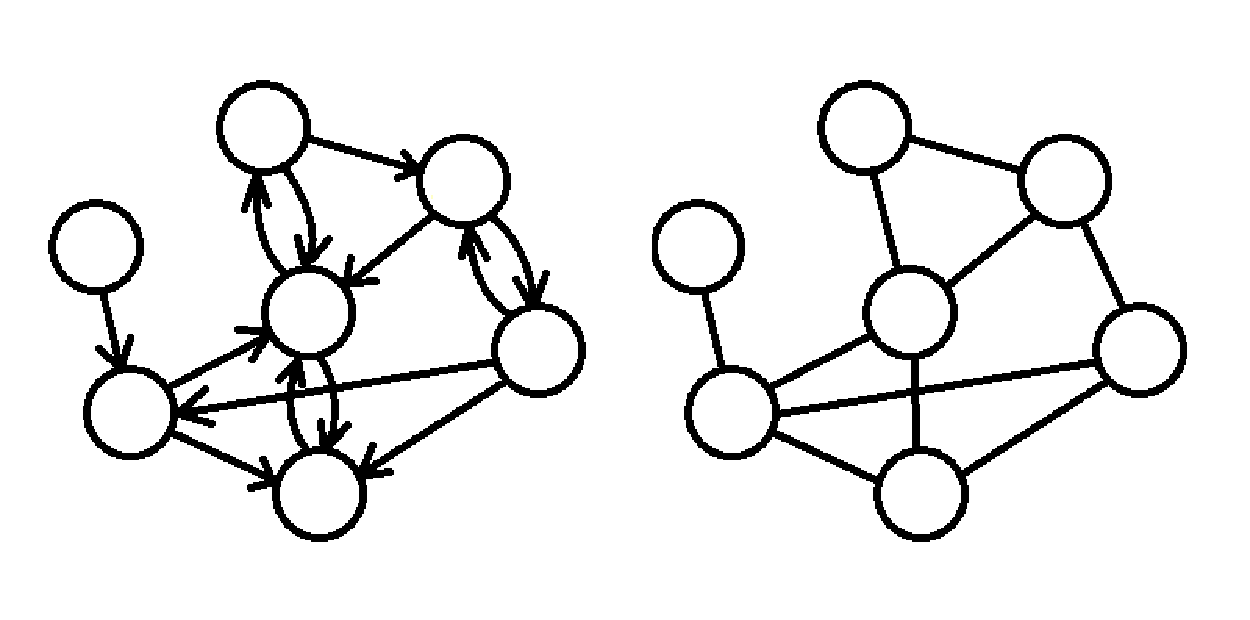
\includegraphics[width=8cm]{image/graph02.pdf}
    }
  \end{exampleblock}
}
    
\subsection{部分グラフ}
\frame{
  \frametitle{部分グラフ}
  \begin{block}{subgraph}
    グラフ$G=(V(G),E(G))$に対して,
    \[ V(H) \subset V(G) ~~ and ~~ E(H) \subset E(G) \]
    となる$H=(V(H),E(H))$をGの\alert{部分グラフ}という.\\
    このとき$G$は$H$を含むともいう.
  \end{block}
}

\frame{
  \begin{exampleblock}{部分グラフの例}
    左が有向グラフ,右が無向グラフ
    \center{
      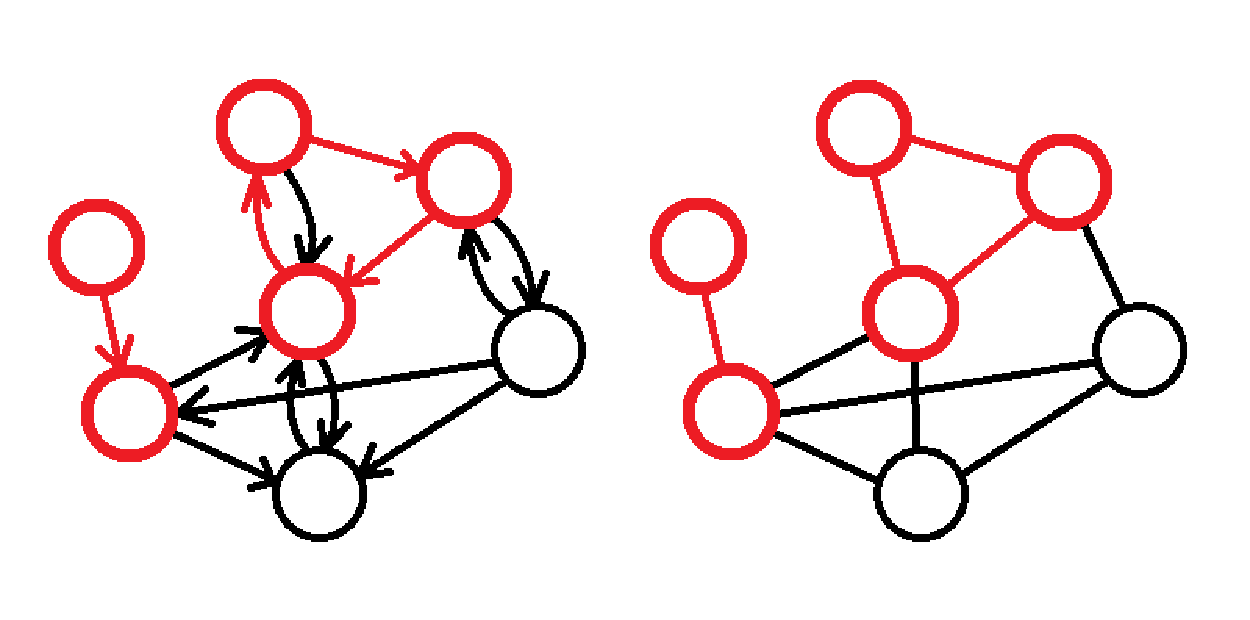
\includegraphics[width=8cm]{image/graph03.pdf}
    }
  \end{exampleblock}
}

\subsection{全点}
\frame{
  \frametitle{全点}
  \begin{block}{spanning}
    グラフ$G$の部分グラフ$H$が,
    \[ V(G) = V(H) \]
    を満たすとき,$H$を$G$の\alert{全点}という.
  \end{block}
}

\frame{
  \begin{exampleblock}{全点の例}
    左が有向グラフ,右が無向グラフ
    \center{
      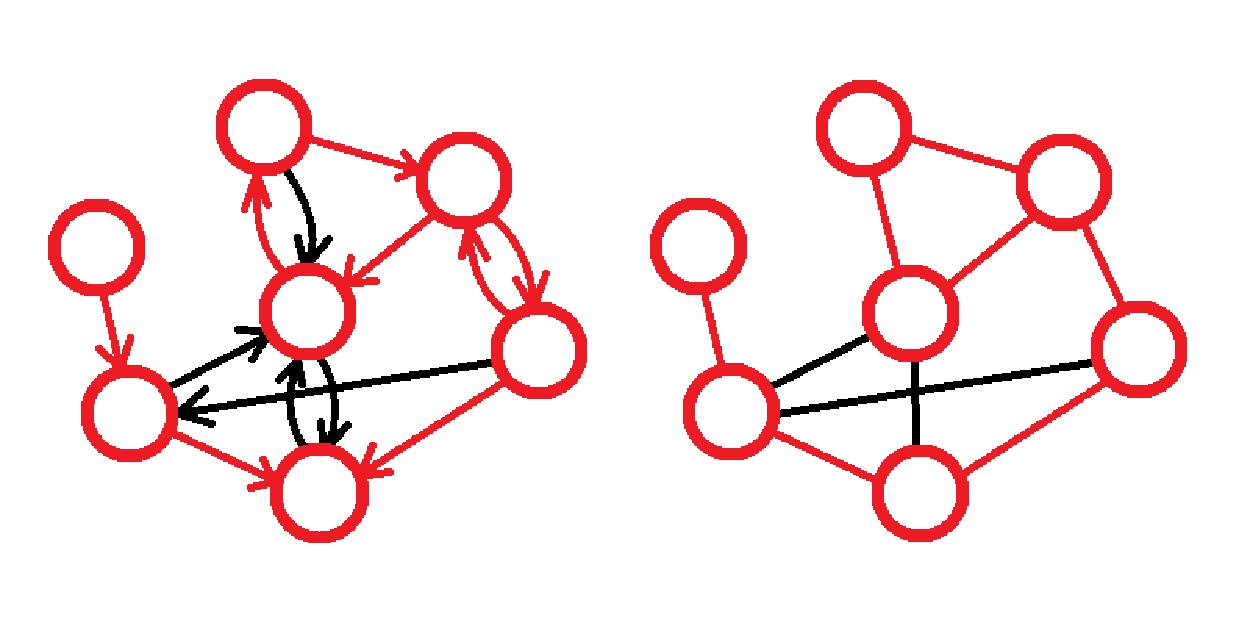
\includegraphics[width=8cm]{image/graph04.pdf}
    }
  \end{exampleblock}
}
    
\subsection{頂点の次数}
\frame{
  \frametitle{頂点の次数}
  \begin{block}{degree}
    無向グラフ$G$と$X,Y \subset V(G), ~ v \in V(G)$に対して,
    \[ E(X,Y) := \{ \{x,y\} \in E(G) : x \in X \backslash Y, y \in Y \backslash X \} \]
    \[ \delta(X) := E(X,V(G) \backslash X) \]
    \[ \delta(v) = \delta(\{v\}) \]
    と定義し,$|\delta(v)|$の値を点$v$の\alert{次数}という.
  \end{block}
}

\frame{
  \begin{block}{degree}
    有向グラフ$G$と$X,Y \subset V(G), ~ v \in V(G)$に対して,
    \[ E^+(X,Y) := \{ \{x,y\} \in E(G) : x \in X \backslash Y, y \in Y \backslash X \} \]
    \[ \delta^+(X) := E^+(X,V(G) \backslash X) \]
    \[ \delta^-(X) = \delta^+(V(G) \backslash X) \]
    \[ \delta(X) = \delta^+(X) \cup \delta^-(X) \]
    と定義し,$|\delta(v)|$の値を点$v$の\alert{次数}という.
  \end{block}
}

\frame{
  \begin{exampleblock}{例のグラフの次数}
    左が有向グラフ,右が無向グラフ
    \center{
      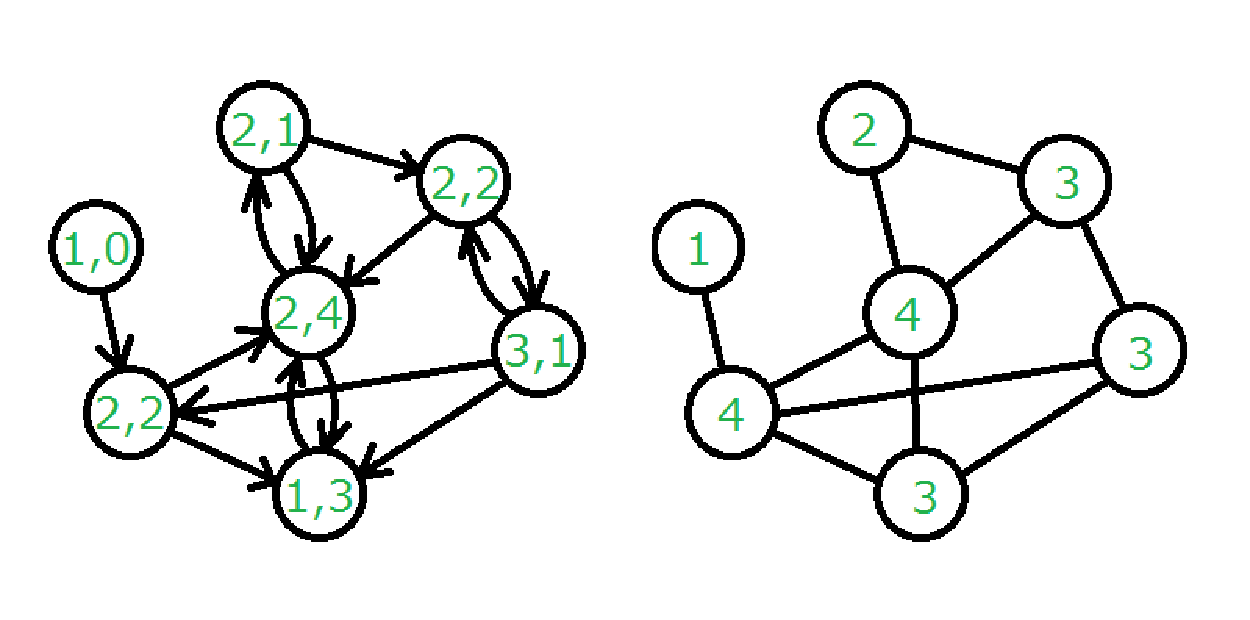
\includegraphics[width=8cm]{image/graph05.pdf}
    }
  \end{exampleblock}
}

\subsection{歩道と道}
\frame{
  \frametitle{歩道と道}
  \begin{block}{walk}
    グラフ$G$に対して,$G$の頂点と辺の有限個の交差系列
    \[ W = v_1, e_1, v_2, \cdots, v_k, e_k, v_{k+1} ~ (k \geq 0) \]
    が全ての$i=1,\cdots k$で$e_i=(v_i,v_{i+1})\in E(G)$\\
    (無向グラフの場合は$e_i=\{v_i,v_{i+1}\}\in E(G)$)を満たすとき,\\
    $W$をGの\alert{歩道}という.
  \end{block}
  \begin{block}{path}
    グラフ$G$に対して,$G$の歩道$W$の頂点がすべて異なるとき,\\
    $W$を$G$の\alert{道}という.
  \end{block}
}

\frame{
  \begin{exampleblock}{道の例}
    左が有向グラフ,右が無向グラフ
    \center{
      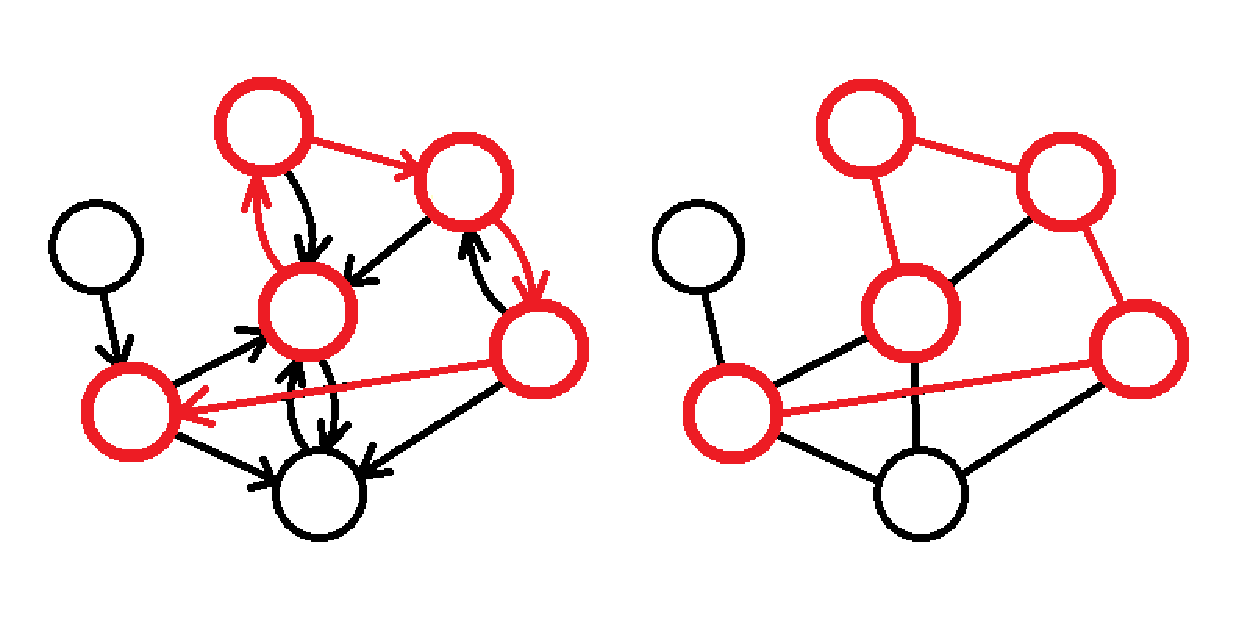
\includegraphics[width=8cm]{image/graph06.pdf}
    }
  \end{exampleblock}
}

\subsection{閉路}
\frame{
  \frametitle{閉路}
  \begin{block}{circuit}
    グラフ$G$の歩道$W = v_1, e_1, v_2, \cdots, v_k, e_k, v_{k+1}$が\\
    $v_1 = v_{k+1}$を満たすとき,$W$を$G$の閉路という.
  \end{block}
}

\subsection{連結}
\frame{
  \frametitle{連結}
  \begin{block}{connected}
    無向グラフ$G$の任意の頂点の組$v,w$について,\\
    $v$と$w$を結ぶ道が存在するとき,$G$は連結であるという.
  \end{block}
}

\frame{
  \begin{exampleblock}{連結グラフと非連結グラフ}
    左が連結グラフ,右が非連結グラフ
    \center{
      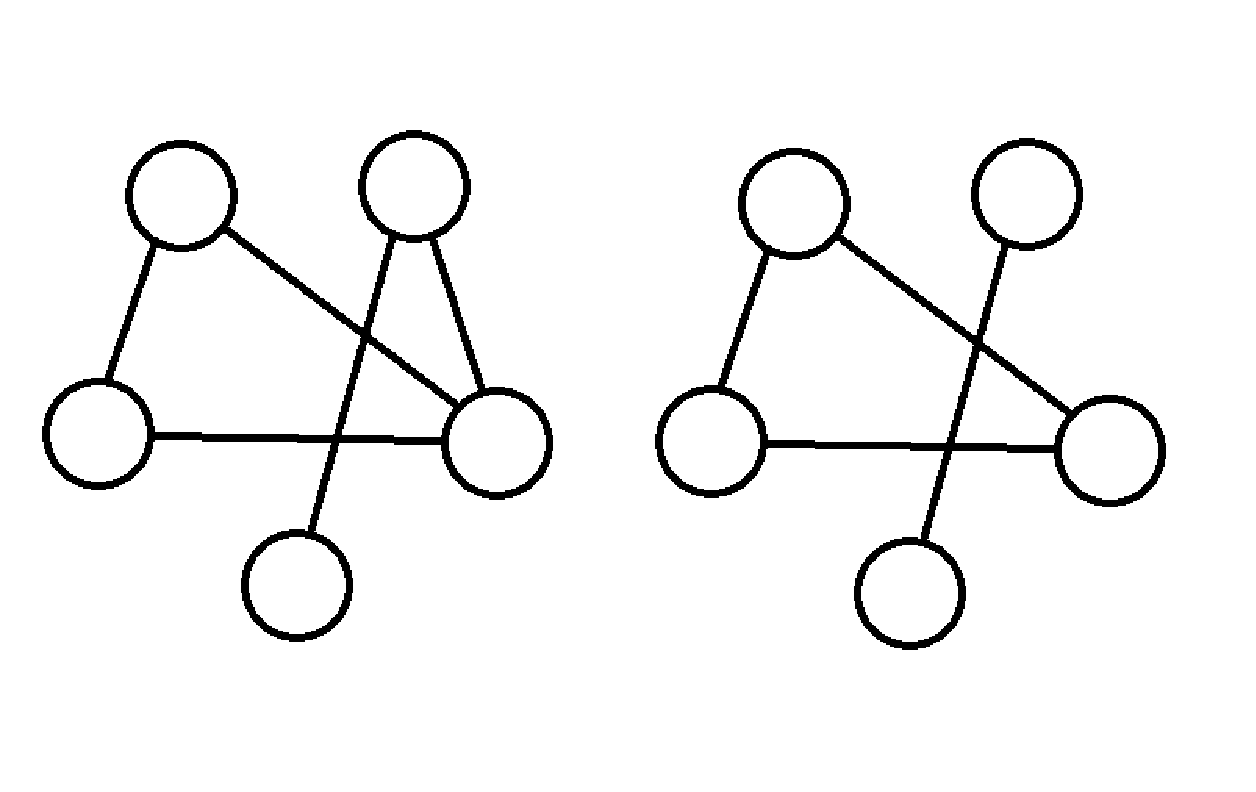
\includegraphics[width=8cm]{image/graph07.pdf}
    }
  \end{exampleblock}
}

\subsection{What's 木?}
\frame{
  \frametitle{木}
  \begin{block}{tree}
    無向グラフ$G$が連結であり閉路が存在しないとき,\\
    $G$を無向木という.
  \end{block}
  \begin{block}{arborescence}
    有向グラフ$G$に閉路が存在せず,1つの頂点を除いて\\
    他の全ての頂点の入次数が1のとき,$G$を無向木という.
  \end{block}
}

\frame{
  \begin{exampleblock}{木の例}
    左が無向木,右が有向木
    \center{
      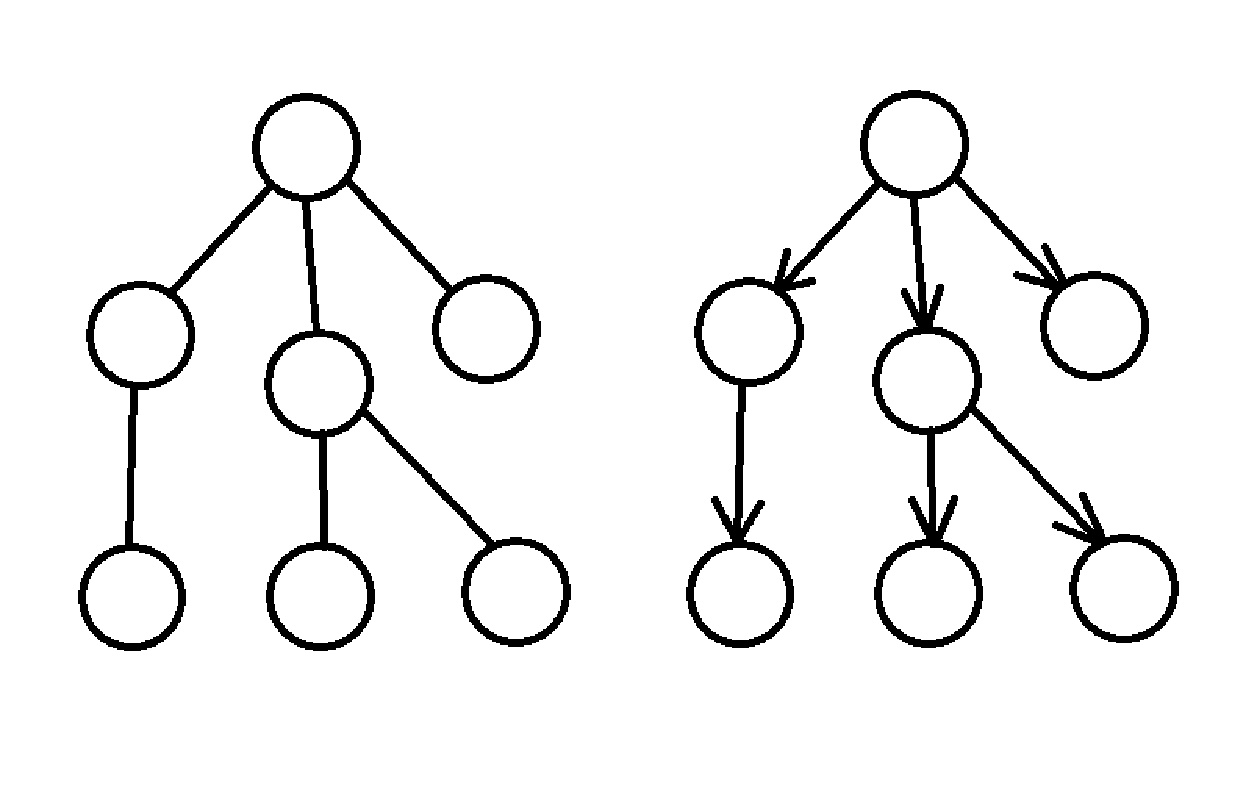
\includegraphics[width=8cm]{image/graph08.pdf}
    }
  \end{exampleblock}
}


\section{木を利用したデータ構造}

\subsection{2分ヒープ}
\frame{
  \frametitle{2分ヒープ}
  \begin{block}{Binary Heap}
    全順序集合$P(C,\leq)$について,$C$上の要素からなるヒープは\\
    以下の操作が実行できる
    \itemize{
    \item push : $O(\log N)$で$C$の要素$x$を追加する
    \item replace : $O(\log N)$で$C$の要素$x$でヒープの最大値をもつ要素を置き換える
    \item pop : $O(\log N)$でヒープの最大値をもつ要素を削除する
    \item delete : $O(1)$で与えられたポインタの先の要素を消去する
    \item top : $O(1)$でヒープの最大値を求める\\
    }
    ヒープ条件を満たす完全二分木の構造\\
    (二分木:出次数が高々2の有向木)\\
    (完全二分木:出次数が0か2で,全ての葉が同じ深さ)
  \end{block}
}

\frame{
  \frametitle{2分ヒープ}
  \begin{alertblock}{ヒープ条件}
    \center{
      全ての要素の値はその親の要素の値より小さいか等しい
    }
  \end{alertblock}
  \begin{exampleblock}{例}
    \center{
      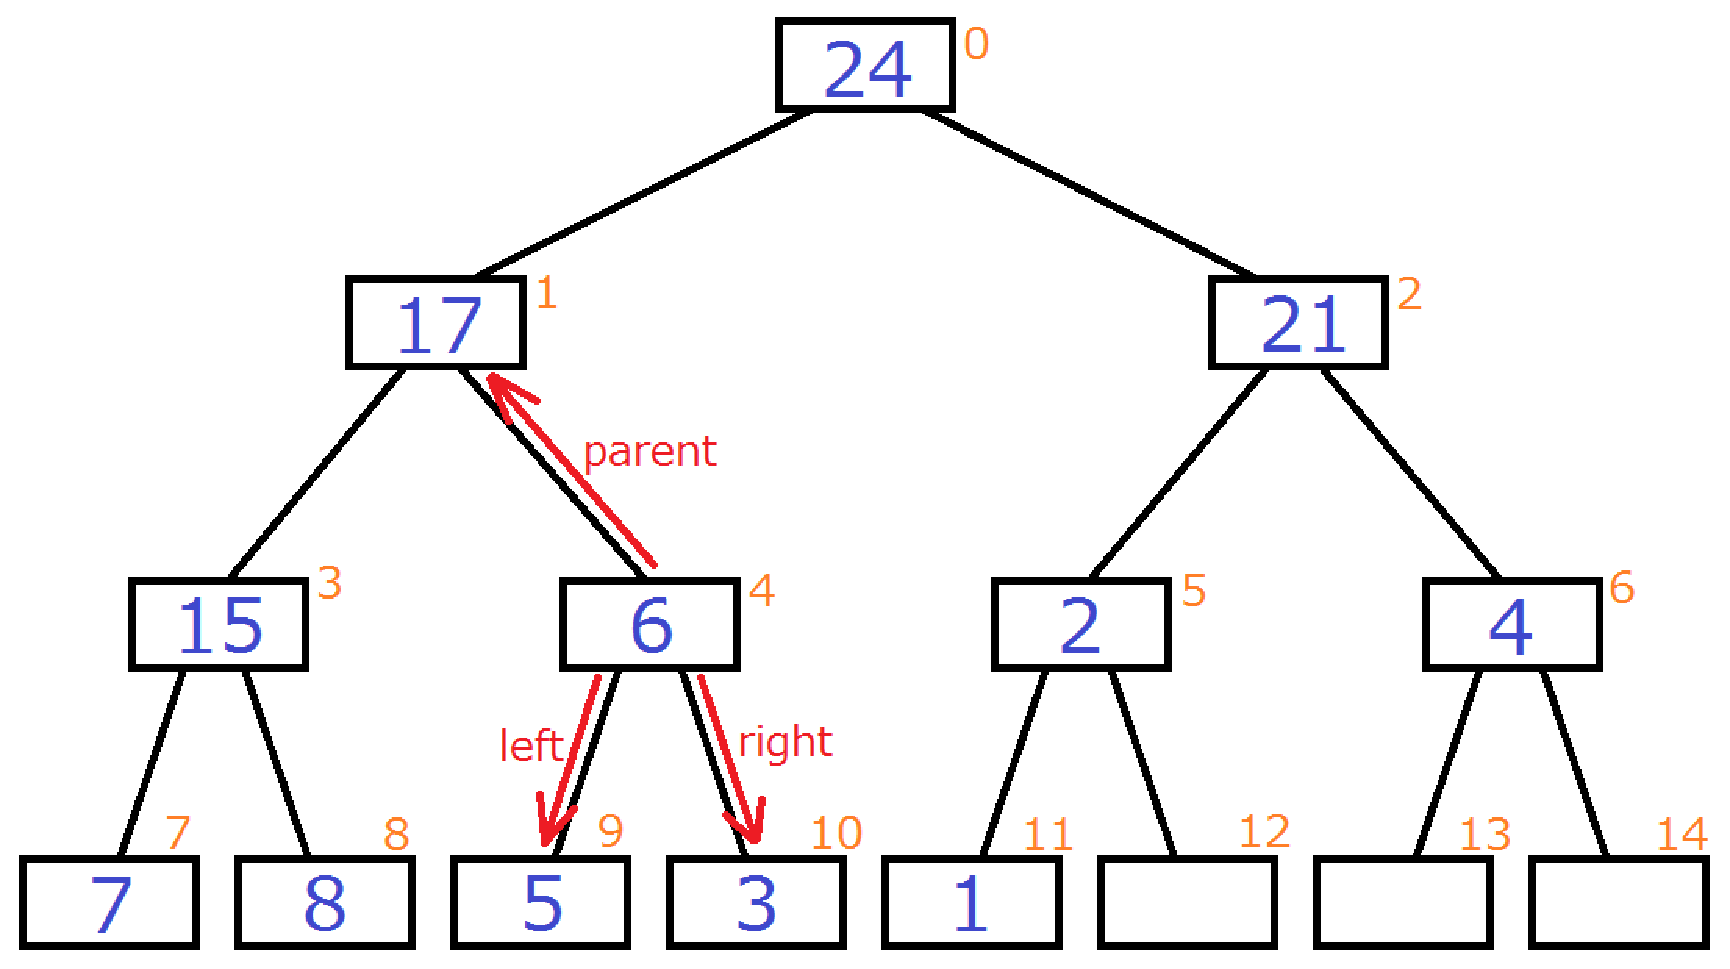
\includegraphics[width=8cm]{image/heap01.pdf}
    }
  \end{exampleblock}
}

\frame{
  \frametitle{push}
  \begin{block}{push}
    \center{
      $O(\log N)$で$C$の要素$x$を追加する
    }
  \end{block}
  \begin{exampleblock}{例}
    \center{
      \includegraphics<1>[width=8cm]{image/heap02.pdf}
      \includegraphics<2>[width=8cm]{image/heap03.pdf}
      \includegraphics<3>[width=8cm]{image/heap04.pdf}
    }
  \end{exampleblock}
}

\frame{
  \frametitle{replace}
  \begin{block}{replace}
    \center{
      $O(\log N)$で$C$の要素$x$ヒープの最大値をもつ要素を置き換える
    }
  \end{block}
  \begin{exampleblock}{例}
    \center{
      \includegraphics<1>[width=8cm]{image/heap05.pdf}
      \includegraphics<2>[width=8cm]{image/heap06.pdf}
      \includegraphics<3>[width=8cm]{image/heap07.pdf}
    }
  \end{exampleblock}
}

\frame{
  \frametitle{pop}
  \begin{block}{pop}
    \center{
      $O(\log N)$でヒープの最大値をもつ要素を削除する
    }
  \end{block}
  \begin{exampleblock}{例}
    \center{
      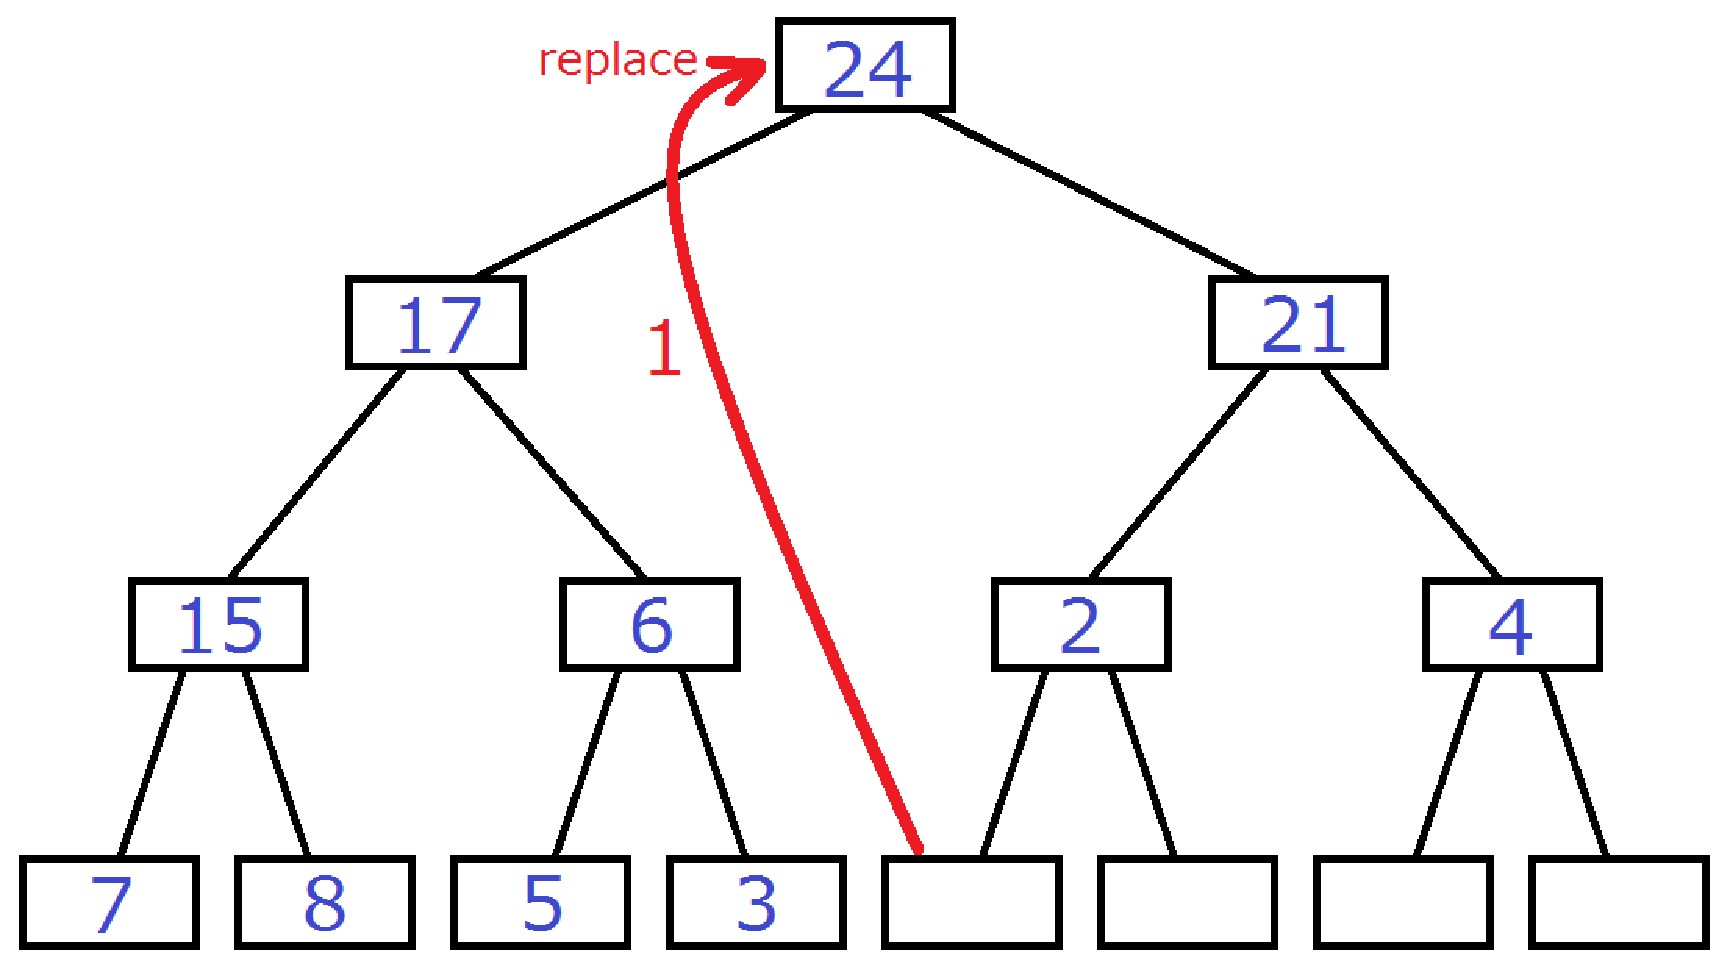
\includegraphics[width=8cm]{image/heap08.pdf}
    }
  \end{exampleblock}
}

\frame{
  \frametitle{delete}
  \begin{block}{delete}
    \center{
      $O(1)$で与えられたポインタの先の要素を消去する
    }
  \end{block}
  \begin{exampleblock}{例}
    \center{
      \includegraphics<1>[width=8cm]{image/heap09.pdf}
      \includegraphics<2>[width=8cm]{image/heap10.pdf}
      \includegraphics<3>[width=8cm]{image/heap11.pdf}
      \includegraphics<4>[width=8cm]{image/heap12.pdf}
      \includegraphics<5>[width=8cm]{image/heap13.pdf}
    }
  \end{exampleblock}
}

\frame{
  \frametitle{top}
  \begin{block}{top}
    \center{
      $O(1)$でヒープの最大値を求める\\ \\
    }
    ヒープの先頭の要素の値が最大値
  \end{block}
  \begin{alertblock}{ヒープは便利!!}
    ヒープを始めとする高速な優先度付きキューはあらゆる場面で活躍する
  \end{alertblock}
}


\subsection{2項ヒープ}
\frame{
  \frametitle{2項ヒープ}
  \begin{block}{Binomial Heap}
    全順序集合$P(C,\leq)$について,$C$上からなる要素の二項ヒープは\\
    以下の操作が実行できる
    \itemize{
    \item top : $O(\log N)$でヒープの最大値を求める
    \item \alert{merge : $O(\log (N+M))$で2つのヒープを併合する}
    \item push : $O(\log N)$で$C$の要素$x$を追加する
    \item pop : $O(\log N)$でヒープの最大値をもつ要素を削除する
    \item delete : $O(\log N)$で与えられたポインタの先の要素を消去する
    \item replace : $O(\log N)$で$C$の要素$x$ヒープの最大値をもつ要素を置き換える\\ 
    }
    ヒープ条件を満たす2項木の集合
  \end{block}
}

\frame{
  \frametitle{2項木}
  \begin{block}{Binomial Tree}
    $B_0$は1個の頂点から構成される.
    $B_k$は2つの$B_{k-1}$から構成され,
    片方の根がもう一方の根の最も左の子になるように連結される.
  \end{block}
  \begin{exampleblock}{例}
    \center{
      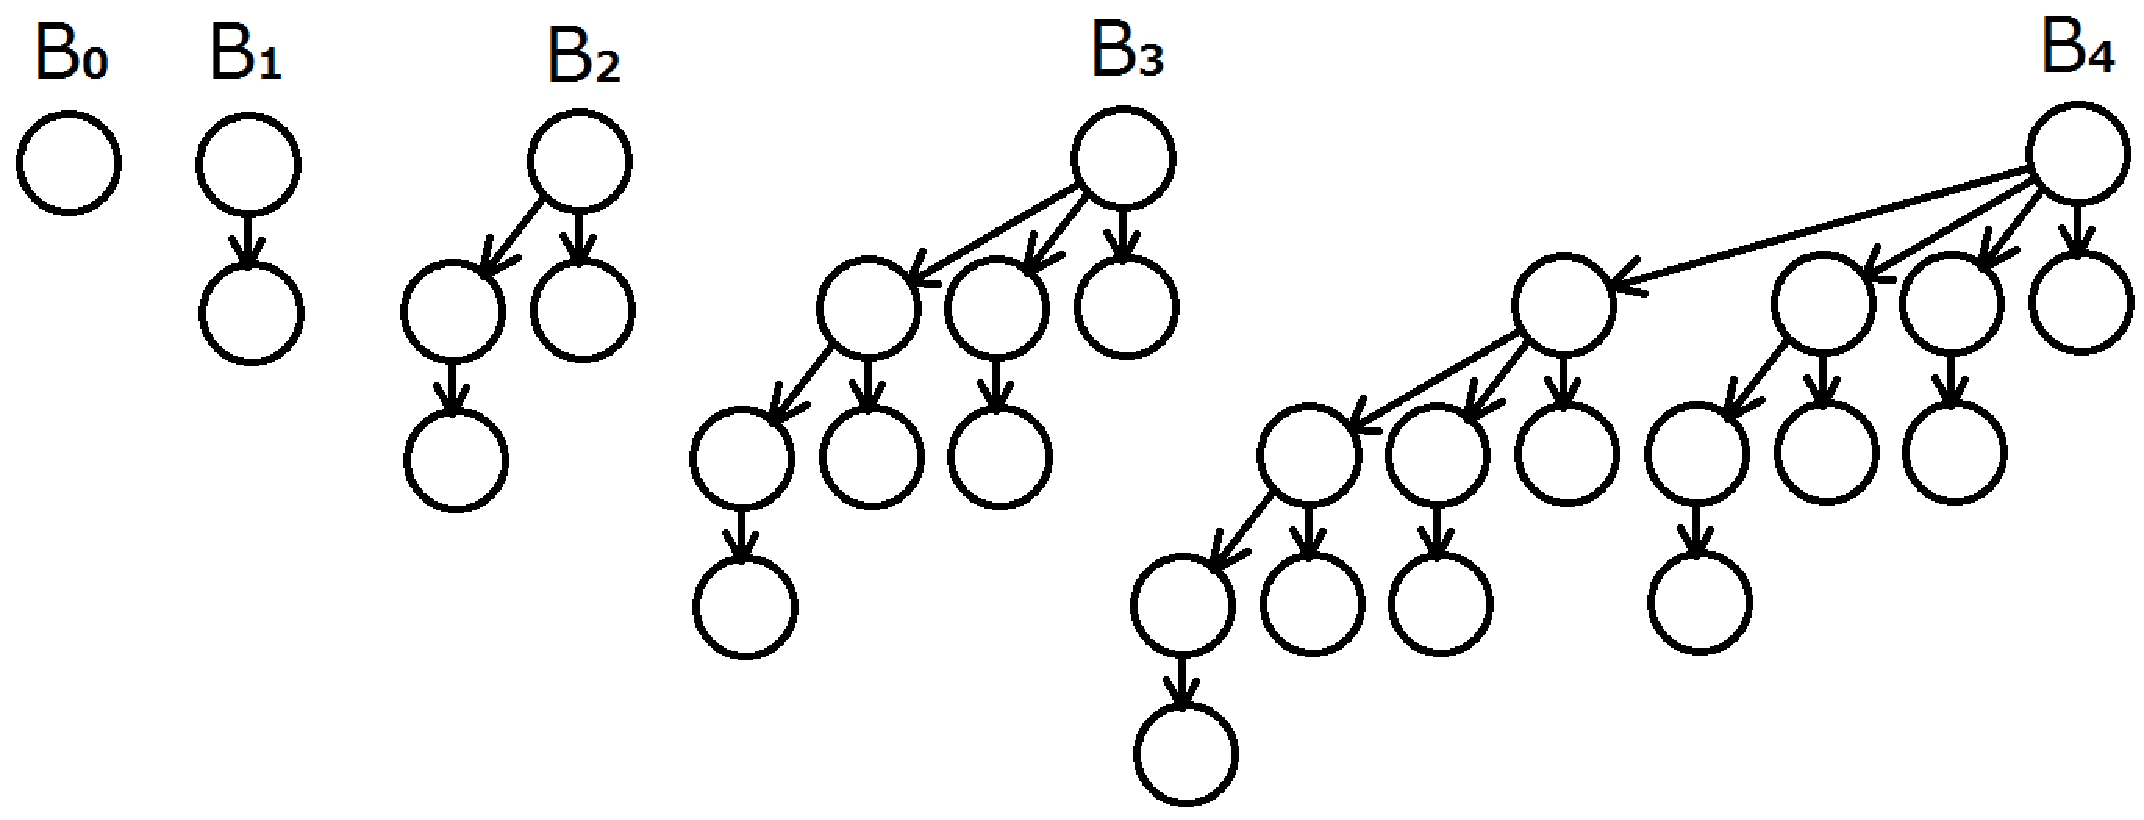
\includegraphics[width=10cm]{image/binomial01.pdf}
    }
  \end{exampleblock}
}

\frame{
  \frametitle{2項木}
  \begin{block}{Binomial Tree}
    各接点は,親を指すポインタ,最も左の子を指すポインタ,\\
    直接右の兄弟を指すポインタを含んでいる.
  \end{block}
  \begin{exampleblock}{例}
    \center{
      \includegraphics<1>[width=10cm]{image/binomial02.pdf}
      \includegraphics<2>[width=3.4cm]{image/binomial03.pdf}
    }
  \end{exampleblock}
}

\frame{
  \begin{block}{Binomial Heap}
    2項ヒープは2項木を小さい順に左から並べた集合として\\
    表現される.
  \end{block}
  \begin{exampleblock}{例}
    \center{
      \includegraphics<1>[width=7cm]{image/binomial04.pdf}
      \includegraphics<2>[width=7cm]{image/binomial05.pdf}
    }
  \end{exampleblock}
}

\frame{
  \frametitle{top}
  \begin{block}{top$(H)$}
    1.  $y \leftarrow$ nil\\
    2.  $x \leftarrow head(H)$\\
    3.  $max \leftarrow -\infty$\\
    4.  {\bf While} $x \neq$ nil {\bf do}\\
    5. ~~ {\bf If} $key[x] > max$\\
    6. ~~~~~ {\bf Then} $max \leftarrow key[x]$\\
    7. ~~~~~~~~~~~~~~ $y \leftarrow x$\\
    8. ~~ $x \leftarrow sibling[x]$\\
    9.  return $y$
  \end{block}
}

\frame{
  \frametitle{top}
  \begin{block}{top}
    各2項木の根の中で最大値を探す.$O(\log N)$
  \end{block}
  \begin{exampleblock}{例}
    \center{
      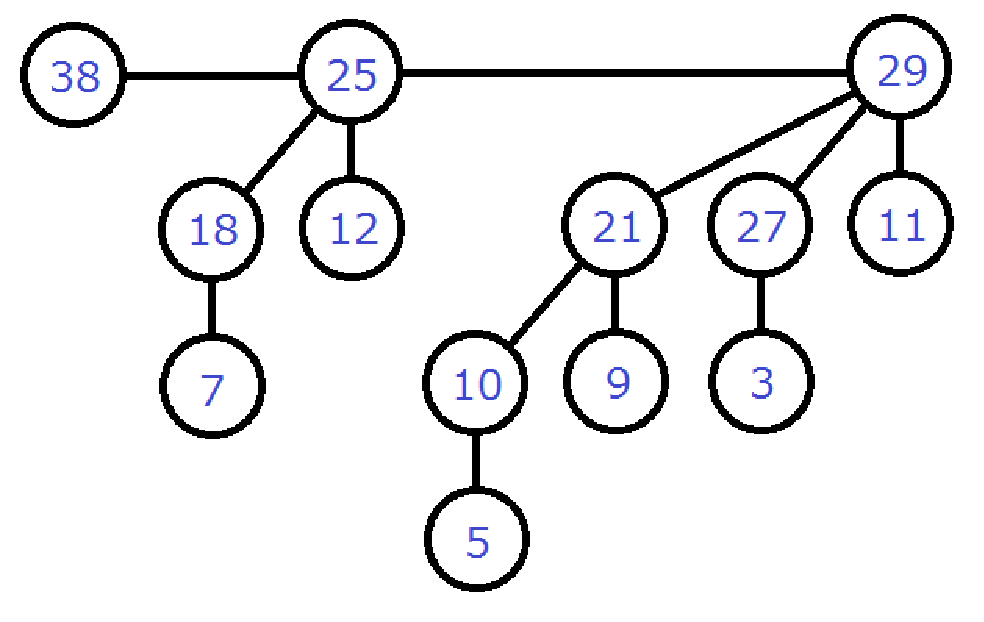
\includegraphics[width=7cm]{image/binomial05.pdf}
    }
  \end{exampleblock}
}

\frame{
  \frametitle{merge}
  \begin{block}{merge$(H_1, H_2)$}
    1.  各2項木を小さい順にmix\\
    2.  $x \leftarrow head(H)$\\
    3.  {\bf While} $sibling(x) \neq$ nil {\bf do}\\
    4. ~~ {\bf If} $deg[x] = deg[sibling(x)] \neq deg[sibling(sibling(x))]$\\
    5. ~~~~~ {\bf Then} $x$と$sibling(x)$の2つの二項木をmerge\\
    6. ~~~~~ {\bf Else} $x \leftarrow sibling(x)$
  \end{block}
  元の$H_1, H_2$は破壊される
}

\frame{
  \only<1-6>{
    \frametitle{merge}
    \begin{block}{merge}
      \only<1>{2つの2項ヒープを併合する}
      \only<2>{2項木を小さい順に併合する}
      \only<3-6>{小さい順に同じサイズのヒープがあれば併合する}
    \end{block}
  }
  \only<7>{
    \frametitle{push}
    \begin{block}{push}
      1要素のみからなる二項ヒープをmergeする
    \end{block}
  }
  \begin{exampleblock}{例}
    \center{
      \includegraphics<1>[width=10cm]{image/binomial06.pdf}
      \includegraphics<2>[width=10cm]{image/binomial07.pdf}
      \includegraphics<3>[width=10cm]{image/binomial08.pdf}
      \includegraphics<4>[width=10cm]{image/binomial09.pdf}
      \includegraphics<5>[width=10cm]{image/binomial10.pdf}
      \includegraphics<6->[width=9cm]{image/binomial11.pdf}
    }
  \end{exampleblock}
}

\frame{
  \frametitle{pop}
  \begin{block}{pop$(H)$}
    1.  $x \leftarrow top(H)$\\
    2.  $H$から接点$x$以下の2項木を除く\\
    3.  $x$の子の$sibling$のリストを逆順に繋ぎ,\\
    ~~~ 出来た2項ヒープを$H'$とする\\
    4.  merge $(H,H')$
  \end{block}
  元の$H_1, H_2$は破壊される
}

\frame{
  \frametitle{pop}
  \begin{block}{pop}
    \only<1>{最大値の要素を調べる}
    \only<2-3>{最大値を消す}
    \only<4-5>{最大値の要素の子だったものを小さい順に併合する}
    \only<6>{残った2つの二項ヒープをmergeする}
  \end{block}
  \begin{exampleblock}{例}
    \center{
      \includegraphics<1>[width=7cm]{image/binomial12.pdf}
      \includegraphics<2>[width=7cm]{image/binomial13.pdf}
      \includegraphics<3>[width=7cm]{image/binomial14.pdf}
      \includegraphics<4>[width=7cm]{image/binomial15.pdf}
      \includegraphics<5-6>[width=7cm]{image/binomial16.pdf}
    }
  \end{exampleblock}
}

\frame{
  \frametitle{delete}
  \begin{block}{delete$(H, x)$}
    1.  $x \leftarrow \infty$\\
    2.  {\bf While} $parent(x) \neq$ nil {\bf do}\\
    3. ~~ $key[x] \leftrightarrow key[parent(x)]$\\
    4. ~~ $x \leftarrow parent(x)$
    5.  $pop(H)$
  \end{block}
  元の$H_1, H_2$は破壊される
}

\frame{
  \frametitle{delete}
  \begin{block}{delete}
    \only<1>{値を$-\infty$に置き換える}
    \only<2>{ヒープ条件を満たすよう調整する}
    \only<3>{pop}
  \end{block}
  \begin{exampleblock}{例}
    \center{
      \includegraphics<1>[width=7cm]{image/binomial17.pdf}
      \includegraphics<2>[width=7cm]{image/binomial18.pdf}
      \includegraphics<3>[width=7cm]{image/binomial19.pdf}
    }
  \end{exampleblock}
}

\frame{
  \frametitle{replace}
  \begin{block}{replace$(H, k)$}
    1.  pop $(H)$\\
    2.  push $(H, k)$
  \end{block}
}

\subsection{フィボナッチヒープ}
\frame{
  \frametitle{フィボナッチヒープ}
  \begin{block}{Binomial Tree}
    全順序集合$P(C,\leq)$について,$C$上からなる要素のフィボナッチヒープは\\
    以下の操作が実行できる
    \itemize{
    \item top : $O(1)$でヒープの最大値を求める
    \item merge : $O(1)$で2つのヒープを併合する
    \item push : $O(1)$で$C$の要素$x$を追加する
    \item pop : $O(\log N)$でヒープの最大値をもつ要素を削除する
    \item size : $O(1)$でヒープの要素数を求める\\
    }
    いいね
  \end{block}
}

\frame{
  \begin{block}{2項木}
    $B_0$は1個の頂点から構成される.
    $B_k$は2つの$B_{k-1}$から構成され,
    片方の根がもう一方の根の最も左の子になるように連結される.
  \end{block}
  \begin{exampleblock}{例}
    \center{
      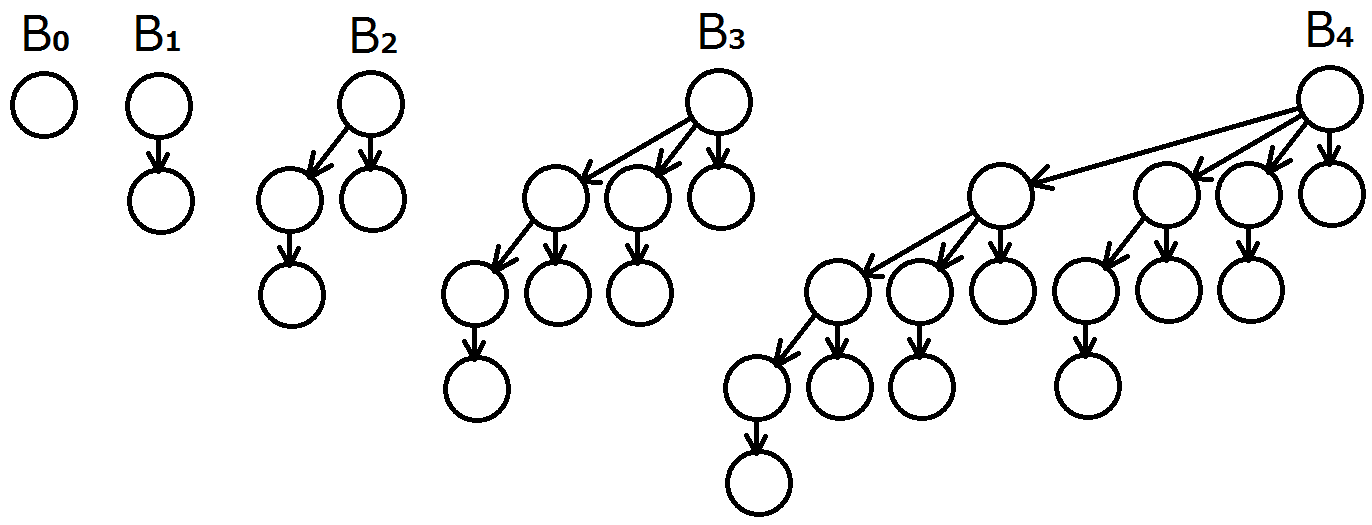
\includegraphics[width=10cm]{image/binomial01.eps}
    }
  \end{exampleblock}
}

\frame{
  \begin{block}{2項木}
    各接点は,親を指すポインタ,最も左の子を指すポインタ,\\
    直接右の兄弟を指すポインタを含んでいる.
  \end{block}
  \begin{exampleblock}{例}
    \center{
      \includegraphics<1>[width=10cm]{image/binomial02.eps}
      \includegraphics<2>[width=3.4cm]{image/binomial03.eps}
    }
  \end{exampleblock}
}

\frame{
  \only<1,2>{
    \begin{block}{2項ヒープ}
      2項ヒープは2項木を小さい順に左から並べた集合として\\
      表現される.
    \end{block}
  }
  \only<3>{
    \frametitle{top}
    \begin{block}{top}
      各2項木の根の中で最大値を探す.$O(\log N)$
    \end{block}
  }
  \begin{exampleblock}{例}
    \center{
      \includegraphics<1>[width=7cm]{image/binomial04.eps}
      \includegraphics<2,3>[width=7cm]{image/binomial05.eps}
    }
  \end{exampleblock}
}

%\subsection{AVL木}
%\subsection{Union-Find Tree}
%\subsection{Segment Tree}
%\subsection{Fenwick Tree}
%\subsection{Wavelet Tree}

%\input{inc/unionfindtree}

\section{グラフアルゴリズム}

\subsection{最小全域木}


\subsection{最短経路問題}
\frame{
  \frametitle{最短経路問題}
  \begin{block}{最短経路問題}
    \begin{itemize}
    \item インスタンス \\
      有向グラフ$G$,重み関数$c:E(G)\rightarrow\mathbb{R}$,2点$s,t\in V$ \\ 
    \item タスク \\
      最短$s-t-$パス$P$ or $s$から$t$が到達不可能であることの決定
    \end{itemize}
  \end{block}
}

%-----------------------------------------------------------

\frame{
  \frametitle{Dijkstraのアルゴリズム}
  単一始点全点間最短距離を求めるアルゴリズム
  \begin{block}{Dijkstraのアルゴリズム}
    \begin{itemize}
    \item 入力 \\
      重み付き有向グラフ$G$\\
      重み関数$c:E(G)\rightarrow\mathbb{R_+}$\\
      始点$s\in V(G)$ \\ 
    \item 出力 \\ $s$から全ての$t\in V(G)$へのパスとその距離
    \end{itemize}
  \end{block}
}

\frame{
  \begin{block}{Dijkstraのアルゴリズム}
    1.  $d(s)\leftarrow 0, \forall v\in V(G)-\{s\}~d(v)\leftarrow\infty, R\leftarrow\emptyset$ で初期化\\
    2.  $d(v)=\displaystyle\min_{w\in V(G)-R}$となる$v\in V(G)-R$を1つ求める\\
    3.  $R\leftarrow R\cup \{v\}$ とする\\
    4.  {\bf For} $(v,w)\in E$ を満たす全ての$w\in V(G)-R$ {\bf do}\\
    ~~~~~ {\bf If} $d(w)>d(v)+c((v,w))$ {\bf then} \\
    ~~~~~~~~ $d(w)\leftarrow d(v)+c((v,w)),~p(w)\leftarrow v$ とする \\
    5.  {\bf If} $R\neq V(G)$ {\bf then} 2に行く
  \end{block}
  $R$は最短路が確定した頂点\\
  2〜5のループは高々$|V(G)|$回
}

\frame{
  \begin{exampleblock}{例}
    \center{
      \includegraphics<1>[width=7cm]{image/dijkstra01.pdf}
      \includegraphics<2>[width=7cm]{image/dijkstra02.pdf}
      \includegraphics<3>[width=7cm]{image/dijkstra03.pdf}
      \includegraphics<4>[width=7cm]{image/dijkstra04.pdf}
      \includegraphics<5>[width=7cm]{image/dijkstra05.pdf}
      \includegraphics<6>[width=7cm]{image/dijkstra06.pdf}
      \includegraphics<7>[width=7cm]{image/dijkstra07.pdf}
      \includegraphics<8>[width=7cm]{image/dijkstra08.pdf}
      \includegraphics<9>[width=7cm]{image/dijkstra09.pdf}
      \includegraphics<10>[width=7cm]{image/dijkstra10.pdf}
      \includegraphics<11>[width=7cm]{image/dijkstra11.pdf}
      \includegraphics<12>[width=7cm]{image/dijkstra12.pdf}
      \includegraphics<13>[width=7cm]{image/dijkstra13.pdf}
    }
  \end{exampleblock}
}

\frame{
  \begin{block}{Dijkstraのアルゴリズム}
    1.  $d(s)\leftarrow 0, \forall v\in V(G)-\{s\}~d(v)\leftarrow\infty, R\leftarrow\emptyset$ で初期化\\
    2.  $d(v)=\displaystyle\min_{w\in V(G)-R}$となる$v\in V(G)-R$を1つ求める\\
                  
    \only<1,2>{\alert{ナイーブな実装では$O(V)$}}
    \only<3,4>{\alert{top,popにかかる時間は$O(\log V)$}}\\
    3.  $R\leftarrow R\cup \{v\}$ とする\\
    4.  {\bf For} $(v,w)\in E$ を満たす全ての$w\in V(G)-R$ {\bf do}\\
    ~~~~~ {\bf If} $d(w)>d(v)+c((v,w))$ {\bf then} \\
    ~~~~~~~~ $d(w)\leftarrow d(v)+c((v,w)),~p(w)\leftarrow v$ とする\\
                    
    \only<3>{\alert{pushで$O(\log V)$}}
    \only<4>{\alert{push,decreasingKeyで$O(1)$}}\\
    5.  {\bf If} $R\neq V(G)$ {\bf then} 2に行く
  \end{block}
  2〜5のループは高々$|V(G)|$回\\
  \only<1,2>{計算量は$O(V^2)$}
  \only<3>{計算量は$O((E+V)\log V)$}
  \only<4>{計算量は$O(E+V\log V)$}
    
  \only<2>{\alert{ここでヒープを使う!!!}}
  \only<3>{\alert{二分ヒープを使った場合}}
  \only<4>{\alert{フィボナッチヒープを使った場合}}
}

\frame{
  \frametitle{Dijkstraのアルゴリズムの利用例}
  \begin{block}{Dijkstraのアルゴリズムの利用例}
    カーナビの経路探索や鉄道の経路案内において利用されている.
    ゲームのAIとか作るのにも使うかも
  \end{block}
}


\section{最後に}

\frame{
  \frametitle{まとめ}
  \begin{itemize}
    \item Light Version なのにスライド61枚もあるのどうするよ
    \item この感じだと完全版は500枚くらいになる!?
    \item 発表時間が5時間くらいあれば・・・
    \item というかそんな膨大なスライド作る時間あんのか
    \item 死ぬしかない
    \item はあ
  \end{itemize}
}

\frame{
  \frametitle{参考文献}
  \begin{block}{参考文献}
    \itemize{
    \item アルゴリズムイントロダクション 第1巻 第2巻
    \item アルゴリズムC++
    \item 組み合わせ最適化 第2版
    \item 計算幾何 理論の基礎から実装まで
    }
  \end{block}
}

\frame{
  \center{
    ご清聴ありがとうございました\\
  }
}


\end{document}
